%-----------------------------------------------------
\section{Digital Scholarly Editing}

\subsection{Theory \parencite{sahleDigitalEdition2016}}
%-----------------------------------------------------
\begin{frame}[allowframebreaks]{What is a Digital Scholarly Edition?}
\metroset{block=fill}\small
Digital editions (as per \cite{sahleDigitalEdition2016}):
        \begin{itemize}
            \item discipline-independent \& not exclusive to text
            \item overcome the limitations of print (financial, inter-/ multimediality, etc.)
            \item follow a digital paradigm like printed editions follow the print paradigm (``shaped by the technical limitations and cultural practices'')
            \item ``A digitised edition is not a digital edition.'' $\to$ it's not about the storage medium (just being on the internet doesn't make it a digital edition!)
            \item ``A digital edition cannot be given in print without significant loss of content and functionality.''
            \begin{itemize}\footnotesize
                \item different views, interactivity, searchability
                \item facsimiles alongside diplomatic transcription and reading versions
                \item all generated from the same source data: \textbf{single source principle} $\to$ How? Data transformation!
                \item $\neq$ Digital Archive,  text corpus or facsimile $\to$ has critical engagement 
            \end{itemize}
        \end{itemize}

\framebreak

We need to start at the beginning: 

\begin{block}{What is a scholarly edition?}
\begin{itemize}
    \item originally stems from ecdotics (\emph{ecdotica, ecdotique, Editorik / Editionswissenschaft}) $\to$ tradition of Philology
    \item \textbf{goal = textual criticism}: reconstruct the original version of a text transmitted to us via textual witnesses (\emph{Lachmannian paradigm})
\end{itemize}
\end{block}

\begin{block}{\cite{sahleDigitalEdition2016}}
    \begin{quote}
        A scholarly edition is the critical representation of historic documents. % \parencite{sahleDigitalEdition2016}. 
        
        \emph{Edition ist die erschließende Wiedergabe historischer Dokumente.}
    \end{quote}
\end{block}

\framebreak 
    
Criteria from \cite{sahleDigitalEdition2016}:
    \begin{enumerate}\footnotesize
        \item \textbf{Representation:} recoding a document and its transformation (in the same or other media)
        \begin{itemize}\scriptsize
            \item Visually: image reproduction, facsimile
            \item Textually: transcription.
            \item varying degrees of closeness/abstraction with regard to the original document
        \end{itemize}
        \item representation $\neq$ presentation
        \item \textbf{Critical engagement} (based on scholarly agenda). ``Critical engagement without representation is not an edition–but an examination, a catalogue or a description.''
        \begin{itemize}\scriptsize
            \item textual criticism
            \item historic criticism
            \item bibliographic criticism
            \item material criticism
            \item visual criticism
            \item etc.
        \end{itemize}
        \item \textbf{Documents:} ``every non-abstract object that is the subject of an edition can be called a document.''
        \item \textbf{Historic:} editions ``explain what is not evident to the present-day reader. In short, they bridge a distance in time, a historical difference. Texts that are created today do not need to be critically edited. They can speak for themselves.''
    \end{enumerate}

\begin{block}{\cite{sahleDigitalEdition2016}}    
    \begin{quote}
        A representation without \lbrack{}critical\rbrack{} treatment or the addition of information is not an edition–but a facsimile, a reproduction or–nowadays–a digital archive or library. 
        
        \textbf{Critical representation} as a compound notion of editing aims at the reconstruction and reproduction of texts and as such addresses their material and visual dimension as well as their abstract and intentional dimension \parencite{sahleDigitalEdition2016}. 
    \end{quote}
\end{block}

\framebreak

Questions to ask if you want to know if it's a Digital Scholarly Edition:
\begin{enumerate}
    \item \textbf{Is there a full representation} of the subject in question?
    \item \textbf{Is it critical?} $\to$ processing rules stated and applied, scholarly knowledge included to make the document easier to understand, regarding material, document genesis/creation, context and reception?
    \item \textbf{Is the edition of academic quality?} $\to$ transparent and rigorous edition process, responsibilities stated, enables future research on a reliable basis.
    \item \textbf{Does the edition follow a digital paradigm?} $\to$ makes use of the possibilities of the digital, not printable without major loss of content or functionality.
\end{enumerate}

\framebreak

\begin{alertblock}{Ideally, a DSE should also implement the FAIR criteria}
\begin{description}\footnotesize
    \item[Findable.] in library catalogs, discovery systems or repositories, with a persistent identifier
    \item[Accessible.] free for any user, no access restrictions? (from open access to usability, language selection, etc.) 
    \item[Interoperable.] data in standardized and widely used format (for example TEI or similar standards), allowing for reuse and data exchange outside of the project. 
    \item[Reusable.] data accessible (individual download, aggregate download, repository, API)? Licenses allowing reuse. Data creation, modelling and processing documented adequately so that others can make sense of it? 
\end{description}
\end{alertblock}

$\to$ \href{https://ride.i-d-e.de/}{RIDE (review journal for digital editions and resources)} \\
$\to$ \href{https://ride.i-d-e.de/reviewers/catalogue-criteria-for-reviewing-digital-editions-and-resources/}{RIDE Criteria for Reviewing Digital Editions and Resources}
\end{frame}

%-----------------------------------------------------

\begin{frame}{Further reading}
    \fullcite{sahleDigitalEdition2016}
    \bigskip 
    
  \begin{block}{Blogpost (short summary)}\footnotesize \href{https://latex-ninja.com/2022/10/30/what-you-really-need-to-know-about-digital-scholarly-editing/}{\emph{What you really need to know about Digital Scholarly Editing}, The \LaTeX{} Ninja Blog, 30.10.2022.} = \parencite{LaTeXNinjaDSE2022}
  \end{block}
    
\end{frame}
%-----------------------------------------------------

\section{Editorial Schools and Workflows}

\begin{frame}{What is a text?}
    Patrick Sahle's text wheel
    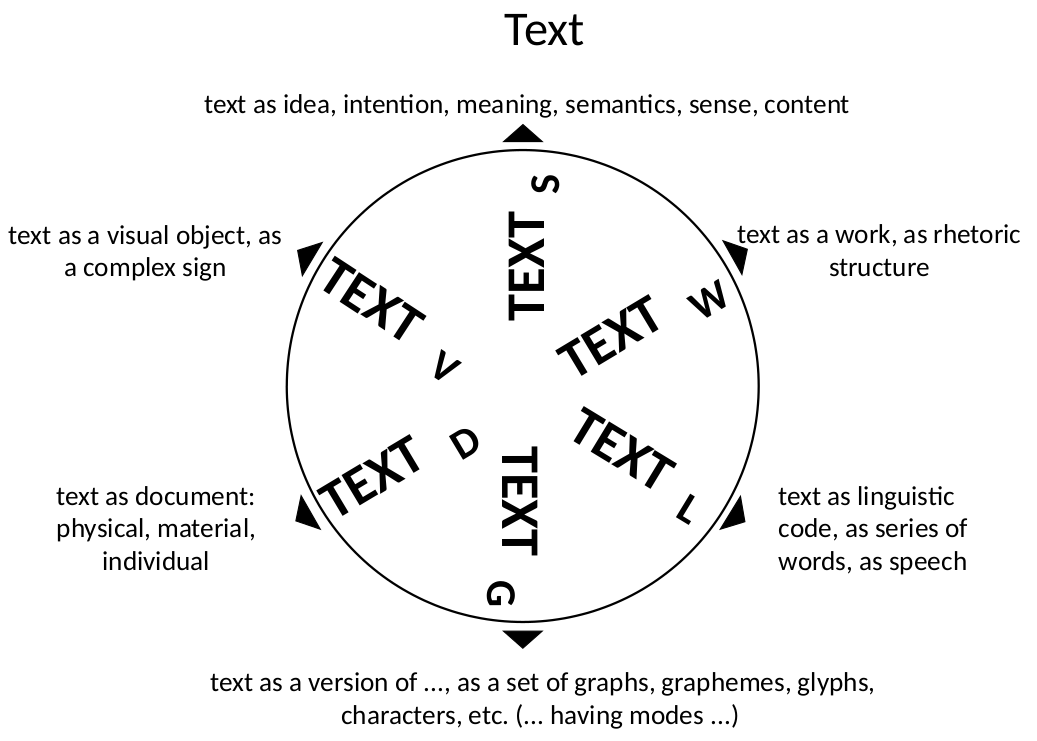
\includegraphics[width=0.95\textwidth]{img/sahle-text-wheel.png}
\end{frame}
%-----------------------------------------------------
\begin{frame}[allowframebreaks]{Edition workflows and schools}
\subsection{Steps involved in DSE}

{\scriptsize
The following slides are adapted from Georg Vogeler's slides on digital editing.
}
\metroset{block=fill}\footnotesize
\begin{columns}
\column{0.65\textwidth}
\begin{block}{Traditional Workflow of Philological Editing}
\begin{itemize}
    \item \textbf{Heuristics:} Find your textual witnesses
    \item \textbf{Transcription:} transfer the text into your prefered alphabet (from the original/from a photo)
    \item \textbf{Collation:} Compare the textual witnesses
    \item \textbf{Recensio:} Evaluate the variants and create a stemma (commenting)
    \item Write your introduction
    \item Typesetting
    \item Create an index (refering to pages)
    \item Print and distribution
\end{itemize}
\end{block}

\column{0.33\textwidth}
\begin{block}{In the digital realm:}
\begin{itemize}
    \item edition 
    \item beta version
    \item just TEI data publication
    \item hybrid (web and print) publication
    \item minimal edition (adaptation from \href{https://go-dh.github.io/mincomp/about}{minimal computing})
\end{itemize}
\end{block}

\alert{A digital edition is social, iterative, a process\dots }
\end{columns}

\framebreak


\begin{columns}
\column{0.48\textwidth}
\begin{block}{„Edition“}
\begin{itemize}
\item  a particular version of a book
\item  a particular version of a product
\item  all the copies of a book that are printed or published at one time
\end{itemize}
\end{block}

\begin{block}{„Historical-critical“ Edition}
\begin{itemize}
\item  Documentation of the history of the text
transmission in the “apparatus of variants”
\item  Critical evaluation of the textual transmission
\end{itemize}
\end{block}

\column{0.48\textwidth}
\begin{block}{Patrick Sahle's text wheel}
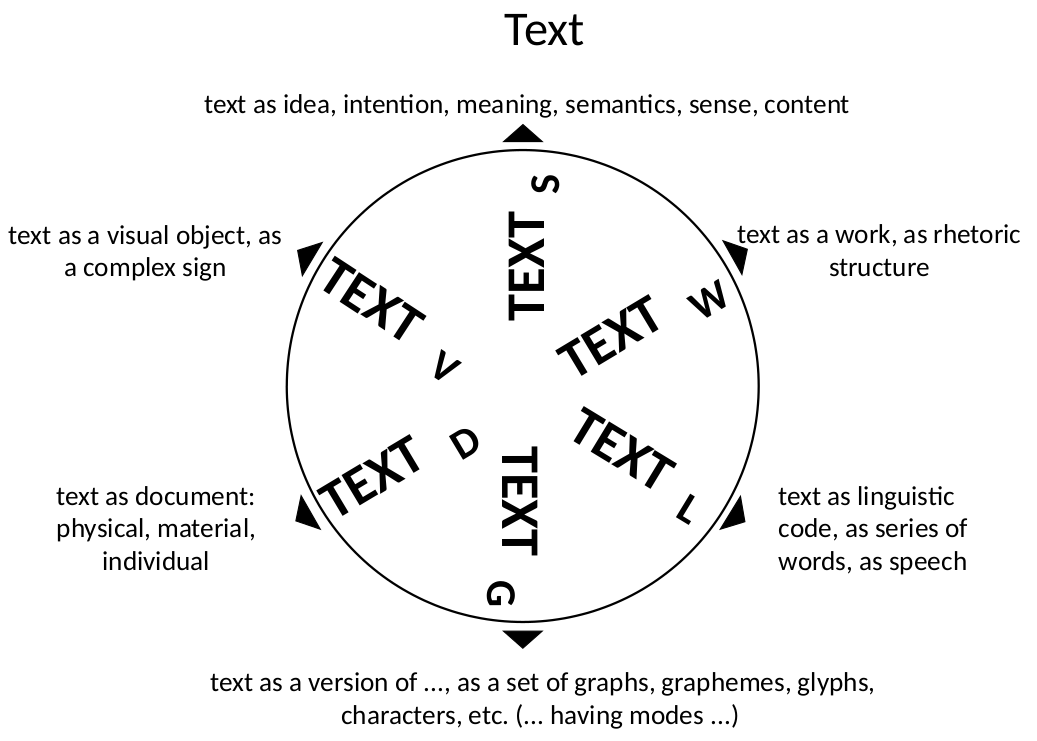
\includegraphics[width=\textwidth]{img/sahle-text-wheel.png}
\end{block}

\begin{block}{Karl Lachmann (1793--1851)}
\textbf{Editorial intervention:} Philological knowledge (linguistics, style) allows us to emend fragmentary textual transmission.
\end{block}
\end{columns}

\framebreak

\begin{block}{Editorial Schools}
\begin{multicols}{2}
\begin{itemize}
\item Lachmann (`Historisch-Kritische Ausgabe', stemmatology)
\item Reading text vs. critical edition = reader-oriented pragmatism / modernised edition / `reading text'
\item  Last authorized edition
\item  First edition / \emph{editio princeps}
\item Main manuscript (Bédier 1937, `Leithandschrift')
\item `diplomatic edition / transcription'
\item Typographic/photographic facsimile
\item `documentary editing' (Tanselle)
\item variorum edition
\item genetic edition / \emph{critique génétique} (Gabler)
\item Copy-Text-Theory (Greg 1950/3, Bowers 1976, 1978)
\item New Philology (Stackmann 1964, 1993, 1994, 1999; Ruh 1978, Cerquiglini 1989)
\end{itemize}
\end{multicols}
\end{block}

\end{frame}




%-----------------------------------------------------

\begin{frame}[standout]

  \alert{If you wanted to practice\dots}
  
  \normalsize
  \href{https://ride.i-d-e.de/reviewers/call-for-reviews/}{Write a RIDE review} on a digital edition \alert{\href{https://ride.i-d-e.de/reviewers/suggested-projects-for-review/}{(suggestions for review)}} according to their \alert{\href{https://ride.i-d-e.de/reviewers/submission-guidelines/}{review criteria}}!
  
  \footnotesize (If you actually plan on submitting, contact the editors first. 2000 words minimum, project from your field. Peer-review can spot things you're unsure about.)
\end{frame}
